% !TEX encoding = UTF-8 Unicode

\documentclass[a4paper]{article}
\usepackage{subcaption}
%\usepackage{hyperref}
\usepackage{color}
\usepackage{url}
\usepackage[T2A]{fontenc} % enable Cyrillic fonts
\usepackage[utf8]{inputenc} % make weird characters work
\usepackage{graphicx}

\usepackage[english,serbian]{babel}
%\usepackage[english,serbianc]{babel} %ukljuciti babel sa ovim opcijama, umesto gornjim, ukoliko se koristi cirilica

\usepackage[unicode]{hyperref}
\hypersetup{colorlinks,citecolor=green,filecolor=green,linkcolor=blue,urlcolor=blue}

%putanja koja radi samo u mom kompjuteru \graphicspath{{/home/max/Pictures/Screenshots}}

%\newtheorem{primer}{Пример}[section] %ćirilični primer
\newtheorem{primer}{Primer}[section]

\begin{document}

\title{Digitalni zvuk\\ \small{Seminarski rad u okviru kursa\\Tehničko i naučno pisanje\\ Matematički fakultet}}

\author{Nina Ostojić, Maksim Krstović, Mihailo Radulović, Dušan Žugić\\ostojic.nina99@gmail.com, maksimusminimus@gmail.com\\ mihailo.radulovic03@gmail.com, dusan.zugic@outlook.com}
\date{15.~novembar 2022.}
\maketitle

\abstract
Cilj ovog seminarskog rada je da na jedan pregledan i koncizan način predstavi opšti uvid u digitalni zvuk, počevši od samog pojma zvuka, kratkog istorijata snimanja, razlika između analognog i digitalnog signala, te ulazi malo detaljnije u proces digitalizacije (odabiranje, kvantizacija i kodiranje), sa osvrtom na snimanje, čuvanje, kompresiju i formate zvuka, da bi na kraju sve bilo zaokruženo podvlačenjem značaja digitalnog zvuka, ciljevima digitalizacije i kako to utiče na sveopštu kulturu i izmenjeno lice sveta.

\tableofcontents

\newpage

\section{Zvuk}

    Zvuk je vibracija koja se širi kroz vazduh (ili neku drugu sredinu) u vidu talasa. Čovek može da čuje zvuk jačine od 16 do 20000 Hz. Ispod ove granice je \textit{infrazvuk}, a iznad \textit{ultrazvuk} (slika~\ref{fig:slika1}). Osnovne karakteristike zvuka su visina, boja i jačina:
    \begin {itemize}
        \item[-] \textit{Visina zvuka} određena je njegovom osnovnom frekvencijom (više tonove stvaraju talasi
        veće frekvencije i obrnuto).
    
        \item[-] \textit{Boja zvuka} je određena karakterom oscilovanja zvučnih talasa. Obično, zvuk nije prost
        harmonijski talas, već je složen iz viših harmonika. Zvuk najniže frekvencije naziva se osnovni ton ili prvi harmonik, a svi ostali su viši harmonici. Složenost talasa, broj i spektar viših
        harmonika određuje boju zvuka. Parni harmonici daju zvuku toplinu i mekoću, a neparni
        oštrinu i hladnoću.
    
        \item[-] \textit{Jačina zvuka} (I) određena je količinom energije koju zvučni talas prenese u jedinici
        vremena kroz jediničnu površinu koja je normalna na pravac prostiranja talasa. Izražava se
        u vatima po kvadratnom metru\cite{10.17632/rwbs7645hg.n}.
    \end{itemize}
  
  \begin{figure}[h]
        \centering
        
        \begin{subfigure}[t]{0.49\textwidth}
            \centering
            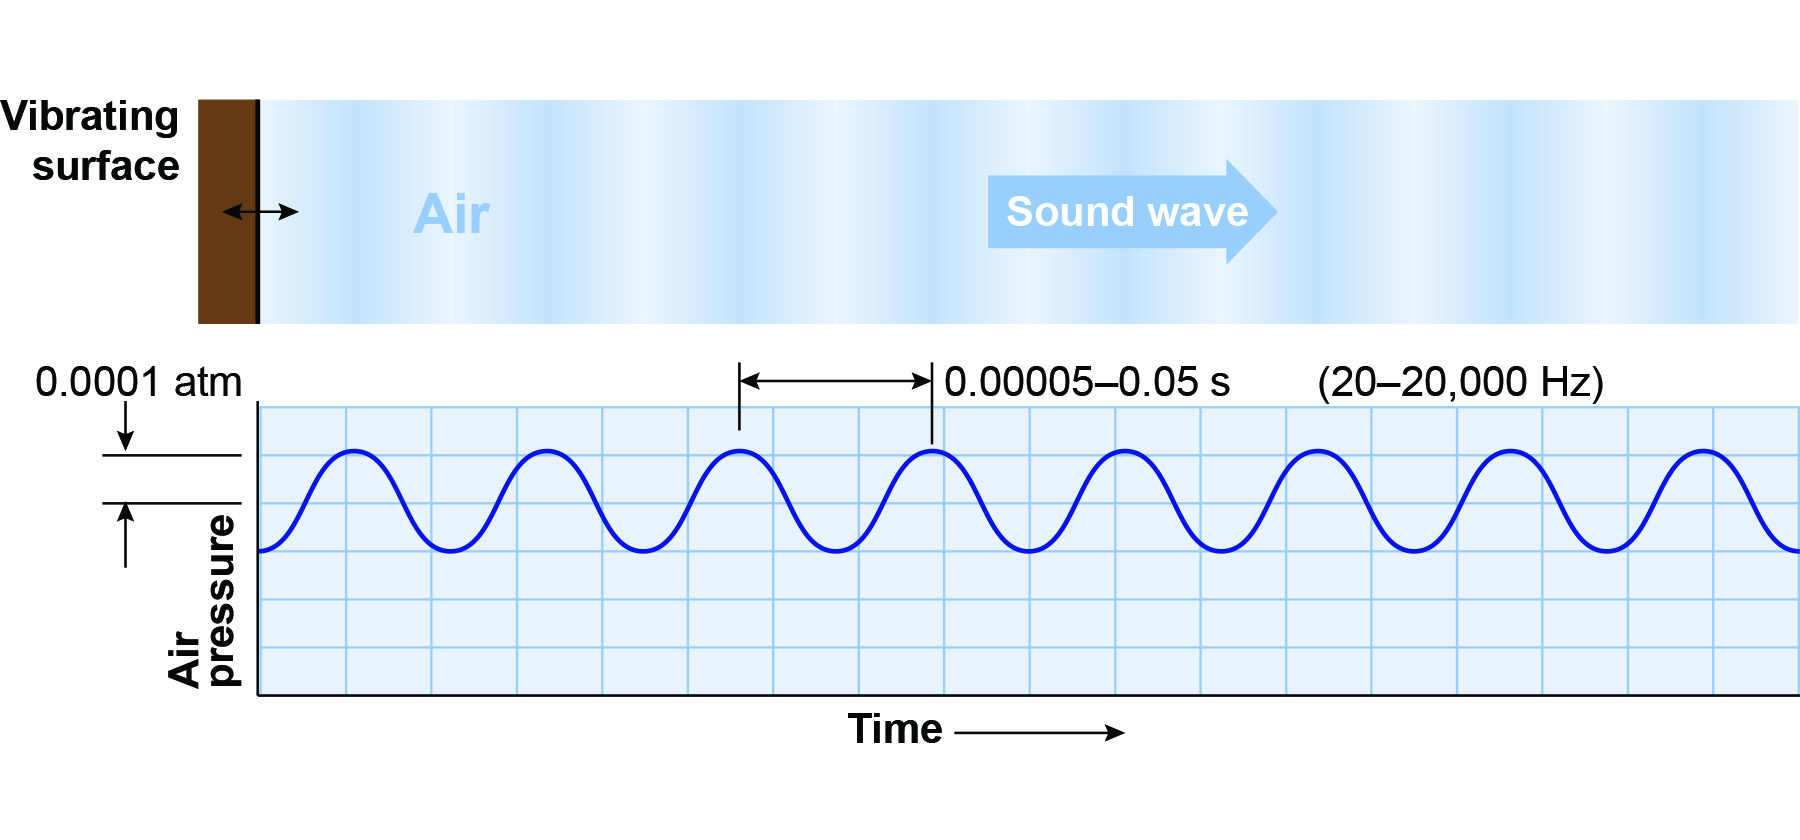
\includegraphics[width=1\textwidth]{airpressure}
        \end{subfigure}
        \caption{Zavisnost vazdušnog pritiska od vremena}
        \label{fig:slika1}
    \end{figure}
  
    \section{Počeci snimanja zvuka}
    Kroz istoriju bilo je mnogo pokušaja da se zvuk snimi, pa da se metode koje su uspele unaprede. Tako smo od analognog snimanja zvuka stigli do digitalnog koji je daleko napredniji. 
    
    \subsection {Analogni zapis zvuka}
    U početku je snimanje zvuka bilo analogno, odnosno, zapisivale su se vibracije koje ljudsko uho prepoznaje kao zvuk na neku vrstu medija. 
    Prvi zvuk je snimljen uz pomoć fonoautografa sredinom 19. veka. Zatim, Emile Berliner je 1889. godine osmislio gramofon koji je mogao da reprodukuje zvuk gotovo 4 minuta. Edison je 1927. patentirao ploču
    koja je mogla da snima 40 minuta zvučnog zapisa, ali se nije proslavio njom. Godine 1928. Fritz Pfleumer je izumeo magnetnu traku i ovaj način snimanja se koristio za vreme Drugog svetskog rata. Nakon toga se pojavila
    stereo magnetna traka koja se mogla koristiti u kućnoj upotrebi. Kompaktna traka i uređaj koji snima i reprodukuje zvuk sa kasete su se pojavili 1964. godine. Kompanija Sony je krajem 80-ih godina predstavila
    novi proizvod DAT (engl.\textit {digital audio tape} ). Ovaj proizvod je prihvaćen od strane raznih industrija jer je mnogo manji od svih prethodnih.
    \subsection {Digitalni zapis zvuka}
    Prvi pokušaj računarske obrade zvuka koji je doveo do uspešne digitalne
    transformacije zvuka desio se početkom 1969. godine u Bel Laboratoriji (\textit {Bell
    Labs}), gde je uspešno proizveden veštački, računarski generisan zvuk. U to vreme su se proizvodili PCM procesori. Oni su pretvarali zvuk u digitalni zapis, pa je napravljen eksperimentalni laserski disk. Zatim, početkom 80-ih, pojavljuju se kompaktni diskovi nepristupačne cene, što se ubrzo menja. Patentirani su kompaktni diskovi (CD-RW) koji imaju mogućnost pisanja i brisanja podataka. Napokon, javlja se uređaj koji može da reprodukuje zapisani zvučni zapis - MP3.

    \section{Digitalizacija zvuka}
    Za razliku od analognog zvuka koji je neprekidni signal u vremenu, digitalni zvuk je isprekidan i postoji samo u određenim trenucima vremena. Digitalizacija se najviše koristi jer su informacije na analognim nosačima zvuka sklone oštećenju reprodukcijom. Za digitalizaciju je potreban računar sa zvučnom karticom i programom za obradu zvuka, zatim uređaji za reprodukciju koji se digitalizuju (gramofon, kasetofon itd.) Radi boljeg kvaliteta dobro je koristiti i dodatnu opremu kao miksetu i pretpojačalo\cite{jurkovic2021digitalizacija}. Digitalizovani zvuk se otprema u jednom od formata: MP3, WAV, AIFF, AAC, OGG i dr.
    
    Da bi se zvuk iz analognog preveo u digitalni oblik potrebno je izvršiti \textit{uzorkovanje}, \textit{kvantizaciju} i \textit{kodiranje}.
    
    \subsection{Odabiranje ili uzorkovanje, semplovanje (engl. \textit{sampling})}
    Uzorkovanje je postupak kojim se uzima vrednost električnog napona signala u određenim trenucima vremena. Što je kvalitet signala bolji, informacija će biti bolje digitalizovana, što znači što je uzorkovanje veće, kvalitetniji će biti dobijeni zvuk. Frekvencija uzorkovanja treba da bude najmanje dva puta veća od najveće frekvencije analognog signala (Nikvist-Šenonova teorema odabiranja). Standardna frekvencija uzorkovanja je 44,1kHz, a može ići i do 192kHz. Opšte prihvaćen CD audio standard je 44.1kHz, DAT kasete (eng. \textit{Digital Audio Tape}) koriste frekvenciju od 48kHz, a zvukovi u igricama 11 ili 22kHz. Može se uzorkovati i na manjim frekvencijama, ali tada će se desiti gubici (na pr. na uzorkovanju od 1kHz dobijeni zvuk će biti neprepoznatljiv - slika~\ref{fig:slika2}). Međutim, što je frekvencija uzorkovanja veća, to je veći i zapis, tj. zauzima više mesta kod čuvanja\cite{jurkovic2021digitalizacija}.
    
    \begin{figure}[h]
        \centering
        \begin{subfigure}[t]{0.49\textwidth}
            \centering
            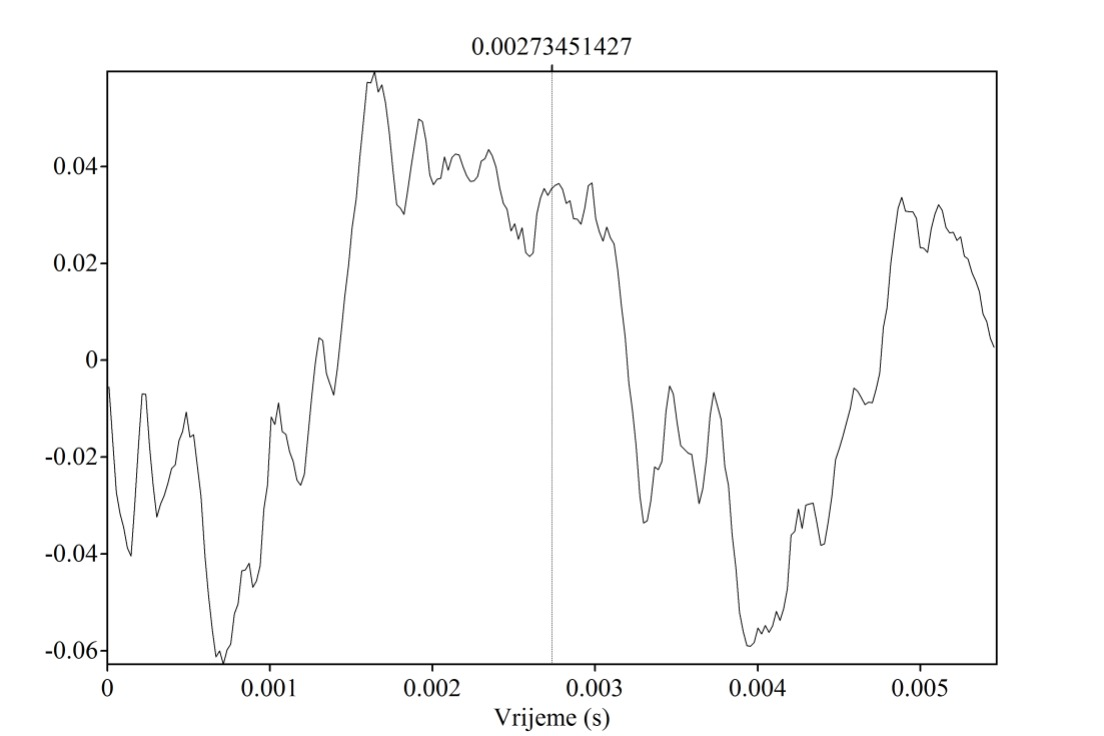
\includegraphics[width=1\textwidth]{Uzorkovanje1}
        \end{subfigure}
        \hfill
        \begin{subfigure}[t]{0.49\textwidth}
            \centering
            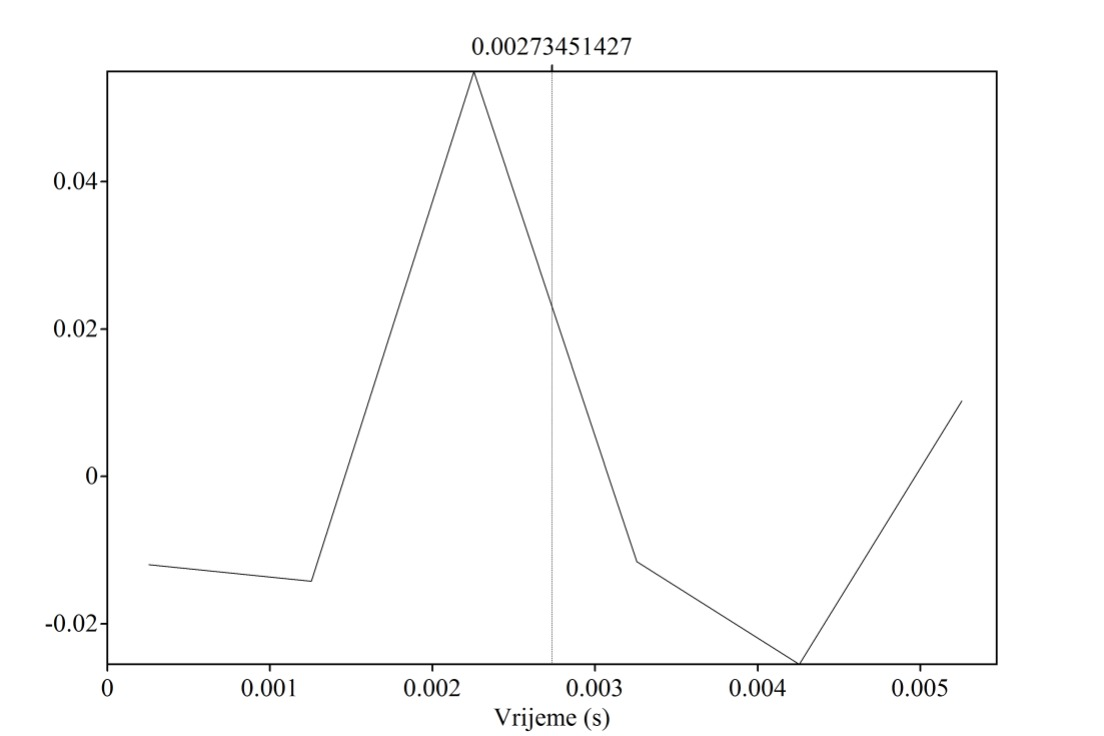
\includegraphics[width=1\textwidth]{Uzorkovanje2}
        \end{subfigure}
        \caption{Uzorkovanje na 44,1kHz i na 1kHz}
        \label{fig:slika2}
    \end{figure}
    
    
    \subsection{Kvantizacija}
    Posle semplovanja ide kvantizacija što je postupak kojim se odabrane vrednosti električnog napona zaokružuju na najbližu od dozvoljenih vrednosti. Pošto jedna sekunda zvučnog zapisa može da se podeli na 44 100 delova (frekvencija uzorkovanja), svaki deo ima amplitudu koja nosi informaciju o zvuku, a ta informacija se prenosi u digitalni oblik, bit. Dubina bita se prikazuje formulom: 2x = n, gde je x broj bitova, a n broj mogućih kombinacija. Kvalitet zvuka direktno proporcionalno zavisi od broja bitova. Za digitalizaciju je standardan 16-bitni prikaz. Tokom kvantizacije neophodno dolazi do kvantizacijske greške (eng. \textit{quantization error}) koja uzrokuje šum u zapisu jer neminovno dolazi do gubitka informacije. Međutim, taj šum se obično ne primećuje\cite{10.17632/rwbs7645hg.2}.
    
    \subsection{Kodiranje}
    Kodiranje (eng. \textit{Encoding}) je niz znakova u digitalnom formatu koji se koriste za prenos i skladištenje. To je i proces pretvaranja podataka u neki drugi format i često se koristi za redukciju veličine audio datoteke. Pri kodiranju svaka vrednost se predstavlja logičkim nulama i jedinicama, tj. bitovima. Broj bitova (8, 16, 24...) određuje dinamički raspon jačine zvuka, što se izražava u decibelima\cite{10.17632/rwbs7645hg.1}. U digitalizaciji (prevođenju analognog u digitalni signal), kao što smo rekli, frekvencija uzorkovanja mora da bude najmanje dva puta veća od najveće frekvencije analognog signala i, zavisno od broja bitova, interval je podeljen na 2n nivoa, te se digitalni signal sastoji od blokova n bitova. Metode kodiranja koje se ovde koriste su:
    \begin{itemize}
        \item \textit{Pulsna kod modulacija} (eng. \textit{Pulse code modulation, PCM}) – intervali su jednako raspoređeni
        \item \textit{Delta modulacija} (eng. \textit{Delta modulation, DM}) – uzorci se ne razlikuju mnogo i potrebno je manje bitova nego kod PCM\cite{10.17632/rwbs7645hg.3}
    \end{itemize}
    Digitalizacija se obavlja u analogno-digitalnom pretvaraču (eng. \textit{A/D converter}). Bitska brzina (eng. \textit{bit rate}) je broj bitova obrađenih u jedinici vremena, tj, u ovom slučaju, koliko je kilobita u sekundi potrebno za smeštanje zvuka (kbps – eng. \textit{kilobit per second}).
    
    \section{Čuvanje digitalnog zvuka}
    Za čuvanje je bitno odrediti koji se kvalitet medijuma traži: kapacitet, dugovečnost, pouzdanost, način rukovanja i naravno, cena kao i dostupnost. Uglavnom se koriste:
    \begin{itemize}
        \item izmenjeni diskovi
        \item tvrdi diskovi
        \item magnetne trake
    \end{itemize}
Od izmenjenih diskova, danas se najviše koriste optički diskovi kao što su CD, DVD, BD koji mogu skladištiti od 800 MB do 50 GB. Oni su jeftini, laki za korišćenje, međutim previše su osetljivi te im je rok trajanje kratak. Stoga se ne preporučuju za dugoročno čuvanje digitalnog zvuka kao ni drugih informacija. 
Tvrdi diskovi mogu biti megnentni i memorijski i razlikuju se po kapacitetu, gde magnetni diskovi mogu skladištiti do nekoliko terabajta. Obe vrste imaju brz pristup informacijama. Magnetni imaju precizne mehaničke delove pa mogu biti osetljivi na habanje vremenom, dok su memorijski diskovi prenosivi i bolje podnose spoljne uticaje. 
Za razliku od diskova, magnetne trake nemaju brz pristup podacima te se sve manje koriste iako su lake za rukovanje.\cite{jurkovic2021digitalizacija} 

        \section{Kompresija i formati audio zapisa}
    MP3 format jedan je od najpoznatijih formata, a ostali poznatiji su WAV, AIFF, AAC,
    OGG i dr. MP3 format dolazi sa određenim gubicima i to je njegova najveća mana ali u isto vreme ima tu prednost manje veličine. Veličina zapisa bude gotovo 1/10 od nekompresovanog zapisa, kao sto su WAV ili AIFF formati koji ne zrtvuju nikoju količinu informacija zarad kompresije. Kvalitet
    MP3 formata zavisi od broja bitova koji će se koristiti, što je veći broj bitova, to je bolji zapis,
    bolji kvalitet. Nasuprot tome, postoje nekompresovani WAV i AIFF formati. To je WAV
    standardni format za snimanje zvučnih zapisa. Koriste se standardne i minimalne
    vrednosti – 44,1 kHz, 16-bitni ekran i dva kanala (tabela~\ref{Tab:tabela1}). AIFF format je veoma sličan WAV formatu.
    S obzirom na to da su oba formata nekompresovana, daju zvuk koji je bogat raznolikošću
    frekvencije, dobijaju se i originalno uzorkovanje i dubina pa su iz navedenih razloga
    lakši za dalju obradu. Njihov najveći nedostatak je veličina, koja može biti između 20-40 Mb po
        zapisu i ponekad nemogućnost razmene zapisa upravo zbog veličine\cite{10.17632/rwbs7645hg.4}.
    

    \begin{table}[ht]
    \centering    
    \begin{tabular}{lll} \hline
    & \textbf{Veličine formata} & \\ \hline
        Stopa uzorkovanja & Nekompresovan WAV & Kompresovan MP3 \\ \hline
        41.4 kHz, 16-bit(CD) & 105.84 MB & 24 MB \\ \hline
        41.4 kHz, 32-bit & 211.68 MB & 46.5 MB \\ \hline
        41.4 kHz, 64-bit & 423.36 MB & 93 MB
    \end{tabular}
    \caption{Veličine formata u trajanju od 10 minuta} 
    \label{Tab:tabela1}
    \end{table}


Zašto kompresovati?
Kompresija se može koristiti za suptilno masiranje zvuka kako bi ona zvučala prirodnije i razumljivija bez dodavanja izobličenja, što rezultira pesmom koja je „udobnija“ za slušanje. Pored toga, mnogi kompresori - i hardverski i softverski - imaće prepoznatljiv zvuk koji se može koristiti za ubrizgavanje divnih boja i tonova u inače beživotne numere na primer. Isto tako, prekomerno kompresovanje određenog fajla može zaista uništiti ideju tog zvuka. Kompresija audio podataka, koju ne treba mešati sa kompresijom dinamičkog opsega, ima potencijal da smanji propusni opseg prenosa i zahteve za skladištenje audio podataka. Algoritmi audio kompresije su implementirani u softver kao audio kodeci. I kod kompresije sa gubicima i bez gubitaka, količina informacija je smanjena korišćenjem metoda kao što su kodiranje, kvantizacija, diskretna kosinusna transformacija i linearno predviđanje kako bi se smanjila količina informacija koje se koriste za predstavljanje nekompresovanih podataka.    
\subsection{Zaštitita digitalizovanog materijala}   
Digitalizovani materijal treba zaštititi od neovlašćenog pristupa, kopiranja i
distribucije, a njenu autentičnost mogu potvrditi mehanizmi zaštite građe. Neki
od metoda zaštite su:
\begin{itemize}
    \item mehanizmi zaštite sistema,
    \item  šifrovanje,
    \item  digitalni potpisi,
    \item  digitalni sertifikati,
    \item  digitalni vodeni žigovi,
    \item  šifrovane koverte 
\end{itemize}
Postoji mnogo mehanizama zaštite sistema i nijedan od njih nije savršen, a jedan od njih je češći
koristi se upravljanje nivoom pristupa. Prilikom uspostavljanja nivoa, to je sad omogućilo
pristup određenim podacima i uslugama, a pristup  nekim drugim je onemogućen. Za pristup se koriste lozinke koje treba da budu tajne i složene da ne mogu svi pristupiti podacima. Dalje, koriste se antivirusne zaštite, ali ih treba redovno održavati. Drugi način zaštite je zaštitni zid.


\section{Ciljevi digitalizacije}
\label{sec:naslovN}

Ciljevi digitalizcije se razlikuju u zavisnosti od toga zašto se primenjuje, želi li se
digitalizacijom zaštititi izvorno gradivo ili omogućiti pristup gradivu. S obzirom na današnju tehnologiju, dolazi se u mogućnost „izrade“ sadržaja kome se može bolje i
jednostavnije pristupiti kroz deljenje sadržaja institucije preko interneta s mnogobrojnim korisnicima istovremeno. Korisnici očekuju aktivno vođenje stranica ustanova i društvenih
mreža kako bi mogli da preslušaju određeni zvučni sadržaj bez fizičkog dolaska u ustanovu.
 
Ustanove digitalizuju svoju građu iz sledećih razloga:

\begin{itemize}
  \item kao plaćenu uslugu,
  \item kako bi dodale novi sadržaj u već postojeću zbirku (npr. priče, legende, bajke i sl.),
  \item vezano za administrativne procese,
  \item zbog izrade internet stranica,
  \item radi konzervacije i restauracije,
  \item zbog ulaganja u nove tehnologije.
\end{itemize}

\subsection{Dobrobiti digitalizacije}
\label{sec:naslovM}

Digitalizacija se danas koristi sve više. Postaje skoro nepojmljivo da određena prodavnica nema bar internet stranicu, dok je to obavezni minimum koji se očekuje od većih kompanija i državnih institucija. Od elektronskih dnevnika, elektronskog bankarstva, društvenih mreža pa sve do muzočkih biblioteka sa milionima pesama, posledice digitalizacije vidimo na svakom koraku. 
Digitalizacija se koristi sve više. Postaje skoro nepojmljivo da određena prodavnica nema bar internet stranicu, dok je to obavezni minimum koji se očekuje od većih kompanija i državnih institucija. Od elektronskih dnevnika, elektronskog bankarstva, društvenih mreža pa sve do muzičkih biblioteka sa milionima pesama, posledice digitalizacije vidimo na svakom koraku. 

Pre digitalizacije, mnogi podaci, informacije, sadržaji su bili znatno skuplji, teže pristupačni, ograničenog broja i upotrebe. Ako bismo hteli da odslušamo novi album određenog izvođača, računar ili telefon je sve što nam je potrebno. Za veliki broj slučajeva, ne bismo morali da platimo, ne bismo imali uslov koliko puta smemo i koliko nas sme da sluša taj sadržaj. 

Izražen primer za prethodno navedene pogodnosti su razne striming(eng. \textit{streaming}) usluge, koje su revolucionisale muzičku industriju. Muzička striming usluga je tip prenošenja i predstavljanja digitalne gradje koja se primarno fokusira na muziku i podkastove(eng. \textit{podcasts}). Zbog jednostavnosti korišćenja, preglednosti i izbora sadržaja skrojenog za određenog korisnika, velika je verovatnoća da ako bismo nekoga pitali kako sluša muziku, odgovor bi bio preko neke striming usluge.
 
Vrlo bitan aspekt digitalizacije je katalogizacija. Zahvaljujući pravilnom arhiviranju i indeksiranju, imamo jasniji pregled i razumevanje sadržaja koje nam štedi vreme pri potrazi za odredjenim podacima, tokom obrade i prilikom rukovođenja\cite{jurkovic2021digitalizacija}.

\section{Zaključak}
\label{sec:zakljucak}

Zvuk su mehaničke vibracije, a čovek prosečnog sluha može da registruje iz intervala 16 - 20 000 Hz. Početkom 19. veka su nastali analogne mašine kojima se mogao zabeležiti zvuk, od kojih je jedan primer gramofon. Upotreba gramofona nije bila preterano skupa, medjutim, ploče preko kojih se čuvao zvuk su bile krhke, osetljive na temperaturu i tokom svakog koriščenja, štetio se reljef i gubili su se podaci. Nakon gramofona, dolazi do izuma magnetne trake, zatim kompaktne trake i konačno optičkih diskova. Optički diskovi se za razliku od prethodno navedenih tehnologija nisu habali tokom reprodukcije i primene, ali je moglo doći do grebanja tokom držanja i neobazrivog rukovođenja.

Zvučni zapisi sa analognih nosača se mogu  zaštititi od propadanja i učiniti dostupnim većem broju korisnika procesom digitalizacije. Digitalizovane zapise možemo spremiti u više formata, a najpoznatiji su MP3, AIFF i WAV. 

Potrebno je digitalizovati građu, pogotovo kulturnu baštinu kako se identitet i kultura ne bi zaboravili i kako bi ljudi, odnosno korisnici, digitalizovanu građu mogli da koriste i tokom celog života. S obzirom na današnju tehnologiju, potrebno je i održavati građu u određenim formatima kako bi bili čitljivi i dostupni većem broju ljudi.
Analogni izvornici ili izvorna digitalna građa će uvek imati svoju vrednost u pogledu informacija, pa i analogni zvuk, jer koliko god pogodnosti digitalni zvuk pružao, naročito u smislu dugotrajnosti i uštede prostora, postoji određeni kvalitet živog zvuka koji se neminovno gubi i koji je za sada nemoguće digitalno reprodukovati.


\addcontentsline{toc}{section}{Literatura}
\appendix

\iffalse
\bibliography{seminarski} 
\bibliographystyle{plain}
\fi

\begin{thebibliography}{9}

\bibitem{10.17632/rwbs7645hg.n} Fizika 4, udžbenik za 4. razred gimnazije, Nataša Čaluković, Krug Beograd   

\bibitem{jurkovic2021digitalizacija} Jurković, Anamaria. Digitalizacija zvuka.  Završni rad, Sveučilište u Zagrebu, Filozofski fakultet, 2021.

\bibitem{10.17632/rwbs7645hg.1} S. Filipović. Digitalizacija zvuka. Računari i programiranje, Wordpress, 2014. on-line at: https://racunariprogramiranje.wordpress.com/2014/02/08/дигитализација-звука/

\bibitem{10.17632/rwbs7645hg.2} Wordpress. Digital Sound and Music. on-line at: http://digitalsoundandmusic.com/5-1-2-digitization/

\bibitem{10.17632/rwbs7645hg.3} Dr. Dheeraj Sanghi. Data Encoding. Computer Networks, Computer Science and Engineering, IIT Kanpur. on-line at: https://www.cse.iitk.ac.in/users/dheeraj/cs425/lec03.html

\bibitem{10.17632/rwbs7645hg.4} S. Filipović. Компресија аудио записа и формати аудио записа. Računari i programiranje, Wordpress, 2014. on-line at: https://racunariprogramiranje.wordpress.com/2013/02/10/компресија-аудио-записа-и-формати-ауд/

\end{thebibliography}

\end{document}
